\documentclass[a4paper, 12pt]{article}
\usepackage[total={17cm,25cm}, top=2.5cm, left=2.5cm, right=2.5cm,  includefoot]{geometry}
\usepackage[utf8]{inputenc}
\usepackage{array}
\usepackage{multirow}
\usepackage{hhline}
\usepackage{gensymb}
\usepackage{graphicx}
\graphicspath{ {} }
\usepackage[czech]{babel}
\usepackage{enumitem}
\usepackage{pdfpages}
\usepackage{amsmath}
\usepackage{verbatim}
\usepackage{listings}
\usepackage{hyperref}
\usepackage{amssymb}


\pagestyle{empty} % vypne číslování stránek




\usepackage[OT2,OT1]{fontenc}
\newcommand\cyr
{
\renewcommand\rmdefault{wncyr}
\renewcommand\sfdefault{wncyss}
\renewcommand\encodingdefault{OT2}
\normalfont
\selectfont
}
\DeclareTextFontCommand{\textcyr}{\cyr}
\def\cprime{\char"7E }
\def\cdprime{\char"7F }
\def\eoborotnoye{\char’013}
\def\Eoborotnoye{\char’003}


\begin{document}



\begin{titlepage}
\begin{center}
\noindent
\Large \textbf{České vysoké učení technické v Praze }\\ Fakulta stavební
\vspace{5cm}

\huge

%vložení loga cvut
\begin{figure}[h!]
	\centering
	
\includegraphics[width=7cm]{logo.png}
\end{figure}

\vspace{0.5cm}

Úvod do zpracování prostorových dat \\

\vspace{3cm}

\Huge  
Ekonomické subjekty\\

\vspace{2cm}

\Large
Bc. Tomáš Klemsa \\
Bc. Petr Poskočil \\
Bc. Robin Pflug \\
Bc. Marek Fáber \\

\end{center}

\end{titlepage}




\pagestyle{plain}     % zapne obyčejné číslování
\setcounter{page}{1}  % nastaví čítač stránek znovu od jedné

\tableofcontents
\newpage

\section{Úvod}
Dokumentace k projektu \textit{Ekonomické subjekty} vypracovaného jako součást předmětu 155UZPR Úvod do zpracování prostorových dat. Autory projektu jsou Bc. Tomáš Klemsa, Bc. Petr Poskočil, Bc. Robin Pflug a Bc. Marek Fáber. Vedoucí předmětu je Ing. Martin Landa, Ph. D. Předmět je zaměřen na zpracování (geo)prostorových dat, geodatabáze, správu geoprostorových dat v objektově-relačních databázových systémech a jejich zpracování.\\
\\
Jako podmínka pro splnění předmětu je vypracování semestrálního projektu, který bude vhodně spjatý se zaměřením předmětu. Jako téma projektu bylo zvoleno propojení ekonomických subjektů s polohovou informací a zjišťování závislosti zániku a vzniku těchto subjektů na spuštění EET.\\
\\
Téma projektu je zvoleno na základě pracovní zkušenosti Bc. Tomáše Klemsy. Projektem vytvořená databáze umožňuje získávat bezplatně jednoduše informace, které jsou v současné době obtížně dostupné a finančně nákladné. SQL dávky jsou zaměřeny na změny týkající se ekonomických subjektů v návaznosti na zavedení elektronické evidence tržeb. 

\section{Zdroje dat}

\subsection{ČSÚ}
Český statistický úřad (ČSÚ) je ústředním orgánem české státní správy a byl zřízen už 8. ledna 1969. Hlavní činností úřadu je získání a zpracování údajů pro statistické účely a jejich poskytnutí dalším státním orgánům, veřejnosti a do zahraničí. Zároveň také koordinuje sběr a zpracování dat údajů prováděných pro jednotlivá ministerstva. Jeho základním posláním je vytvářet objektivní a ucelený obraz ekonomického, sociálního, demografického a ekologického vývoje České republiky a jejích částí.\\
Všechna data a informace jsou na serveru zdarma pro státní správu i běžného uživatele. Data jsou většinou k dispozici ve dvou formátech - ve formátu XML a CVS.[1]

\subsubsection{ČSÚ - NACE}
NACE je akronym pro statistickou klasifikaci ekonomických činností, kterou používá Evropská unie (resp. Evropská společenství) od roku 1970. NACE vytváří rámec pro statistická data o činnostech v mnoha ekonomických oblastech (např. ve výrobě, zaměstnanosti, národních účtech).\\
Statistiky, které vzniknou za použití klasifikace NACE, lze srovnávat v celé Evropské unii. S nižší mírou podrobnosti (na vyšších úrovních) je možné srovnání i se světovými statistikami. Používání NACE je povinné pro všechny členské státy Evropské Unie. 

\begin{figure}[h!]
	\centering
	
\includegraphics[width=8cm]{csu.jpg}
	\caption{Logo ČSÚ [1]}
\end{figure}

\subsection{ČÚZK - RÚIAN}
V polovině roku 2012 byl úspěšně spuštěn provoz systému základních registrů veřejné správy ČR. Jeden ze čtyř základních registrů je i registr územní identifikace, adres a nemovitostí (RÚIAN). RÚIAN je veřejný seznam, který umožňuje uživatelům z řad veřejné, ale i komerční a akademické sféry, dálkový přístup přes internet - aplikace Veřejného dálkového přístupu (VDP) k datům RÚIAN je dostupná zdarma a bez registrace.[2]

\subsubsection{VDP}
Aplikace Veřejný dálkový přístup k datům RÚIAN (VDP) umožňuje nahlížet a získávat data základního registru RÚIAN a také některá data editačního agendového informačního systému územní identifikace (ISÚI) a informačního systému katastru nemovitostí (ISKN). Pro přístup do aplikace VDP není potřeba žádné registrace. Poskytovaná data z VDP jsou zdarma. Data poskytovaná prostřednictvím VDP nejsou referenční, mají pouze informativní charakter.[2]

\subsubsection{Služby}
V rámci Informačního systému základních registrů (ISZR) fungují čtyři základní registry veřejné správy. Zajišťováním provozu ISZR a správou eGON služeb základních registrů se zabývá Správa základních registrů (SZR). eGon služby základních registrů poskytující referenční údaje ze základních registrů i služby poskytující zprostředkované údaje z jiných registrovaných Agendových informačních systémů (AIS). Webové služby ISZR slouží pouze pro komunikaci registrovaných AIS veřejné správy se základními registry.
Služby jsou publikované na vnějším rozhraní systému základních registrů.[2]

\subsubsection{VFR}
Jednou z forem poskytování dat RÚIAN je jejich předávání ve formě souborů obsahujících data RÚIAN nebo ISÚI ve výměnném formátu RÚIAN (VFR). VFR jsou poskytovány ve formátu GML 3.2.1.\\
\textit{Soubory VFR je možné stahovat:}
\begin{itemize}
\item prostřednictvím aplikace Veřejný dálkový přístup (VDP) – volně dostupné pro všechny
\item z internetových (URL) adres vrácených službami ISZR ruianSouboryDat a ruianSouboryZmen – dostupné pouze orgánům státní správy a samosprávy
\end{itemize}[2]

\subsubsection{CSV}
Další formou poskytování údajů je seznam adresních míst RÚIAN ve formátu CSV. Soubory jsou rozděleny po obcích a jsou generovány měsíčně ze stavového VFR.[2]

\begin{figure}[h!]
	\centering
	
\includegraphics[width=8cm]{cuzk.jpg}
	\caption{Logo ČÚZK [2]}
\end{figure}

\section{Software}
Pro tvorbu databáze a prostorových dotazů byl využit open-source software PostgreSQL. Ke stažení dat byl vytvořen skript v programovacím jazyce Python.

\subsection{PostgreSQL}
PostgreSQL je univerzální a objektově relační systém správy databází, nejpokročilejší open-source databázový systém. PostgreSQL byl vyvinut na základě POSTGRES 4.2 na Berkeley Computer Science Department , University of California.\\
PostgreSQL byl navržen tak, aby fungoval na platformách typu UNIX. PostgreSQL byl však také navržen tak, aby byl přenosný, aby mohl běžet na různých platformách, jako jsou Mac OS X, Solaris a Windows.\\
PostgreSQL je bezplatný a open source software. Jeho zdrojový kód je k dispozici pod licencí PostgreSQL, liberální licence s otevřeným zdrojovým kódem. Můžete libovolně používat, upravovat a distribuovat PostgreSQL v jakékoli formě.[3]\\

\begin{figure}[h!]
	\centering
	
\includegraphics[width=8cm]{PSQL.jpg}
	\caption{Logo PostgreSQL [3]}
\end{figure}

\subsection{Python}
Python je vysokoúrovňový skriptovací programovací jazyk, který v roce 1991 navrhl Guido van Rossum. Nabízí dynamickou kontrolu datových typů a podporuje různá programovací paradigmata, včetně objektově orientovaného, imperativního, procedurálního nebo funkcionálního.\\
Python je vyvíjen jako open source projekt, který zdarma nabízí instalační balíky pro většinu běžných platforem (Unix, MS Windows, macOS, Android); ve většině distribucí systému GNU/Linux je Python součástí základní instalace.[4]

\begin{figure}[h!]
	\centering
	
\includegraphics[width=8cm]{python.png}
	\caption{Logo python [4]}
\end{figure}

\section{Praktická část}

\subsection{Stažení dat}
Data byla získána z Registru Ekonomických Subjektů (RES), klasifikace ekonomických činností (CZ-NACE) a Registru Územní Identifikace, Adres a Nemovitostí (RÚIAN). Skriptem v jazyce Python byly na základě \textit{URL id} iterativně stažena všechna potřebná data z webové aplikace českého statistického úřadu. Data byla ukládána do textového souboru. Celkové množství stažených záznamů je přibližně 7 milionů, některé záznamy jsou prázdné.

\begin{figure}[h!]
	\centering
	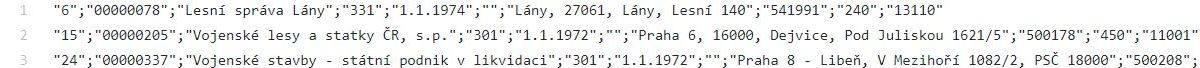
\includegraphics[width=16cm]{data.jpg}
	\caption{Ukázka části textového souboru se staženými daty}
\end{figure}

\subsection{Tvorba tabulek}
Tvorba databáze byla realizována na serveru $geo102.fsv.cvut.cz$ v databázi pgis\underline{ }uzpr pod názvem uzpr20\underline{ }g. Všech pět tabulek bylo vytvořeno SQL skriptem v příkazovém řádku prostřednictvím PostgreSQL. Plnění dat do tabulek zajišťují příkazy obsažené v souboru typu Linux Shell Commands.

\begin{figure}[h!]
	\centering
	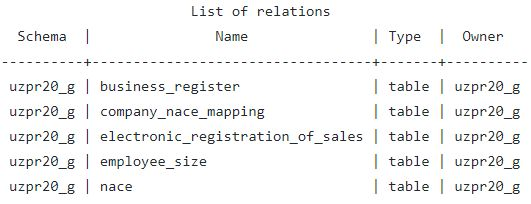
\includegraphics[width=8cm]{schema.jpg}
	\caption{Přehled vytvořených tabulek}
\end{figure}

\newpage
Po vytvoření tabulek s ekonomickými subjekty byly připojeny polohové informace. Polohové informace byly získány z RÚIAN na základě variací společných atributů s ČSÚ. Pouze 2,6\% subjektů zůstaly bez přiřazené polohové informace. 

\subsection{Struktura databáze}
\subsubsection{Tabulka business register}
\begin{itemize}
\item \textbf{id:} číslo záznamu v tabulce
\item \textbf{identification\_number:} identifikační číslo ekonomického subjektu
\item \textbf{company\_name:} název ekonomického subjektu
\item \textbf{legal\_form:} kód právní formy organizace
\item \textbf{establishment:} datum vzniku ekonomického subjektu
\item \textbf{dissolution:} datum zániku ekonomického subjektu
\item \textbf{adress:} adresa ekonomického subjektu
\item \textbf{basic territorial unit:} základní územní jednotka ekonomického subjektu
\item \textbf{employee\_size:} kód kategorie počtu zaměstnanců ekonomického subjektu
\item \textbf{institutional\_sector:} institucionální sektor ekonomického subjektu
\item \textbf{adress\_point:} adresní bod ekonomického subjektu
\end{itemize}

\begin{figure}[h!]
	\centering
	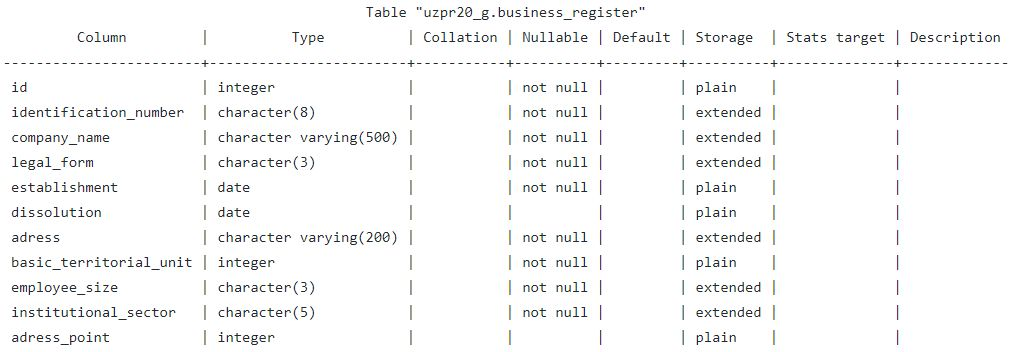
\includegraphics[width=14cm]{br_tab.jpg}
	\caption{Tabulka business register}
\end{figure}

\subsubsection{Tabulka company nace mapping}
\begin{itemize}
\item \textbf{identification\_number:} identifikační číslo ekonomického subjektu
\item \textbf{nace\_code:} kód názvu ekonomické činnosti
\end{itemize}

\begin{figure}[h!]
	\centering
	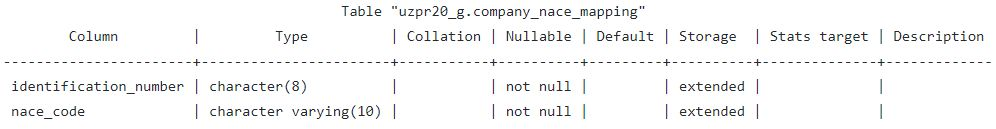
\includegraphics[width=14cm]{nace_tab.jpg}
	\caption{Tabulka company nace mapping}
\end{figure}

\subsubsection{Tabulka electronic registration of sales}
\begin{itemize}
\item \textbf{nace:} kód názvu ekonomické činnosti
\item \textbf{start\_date:} datum spuštění EET
\item \textbf{end\_date:} datum ukončení EET
\end{itemize}

\begin{figure}[h!]
	\centering
	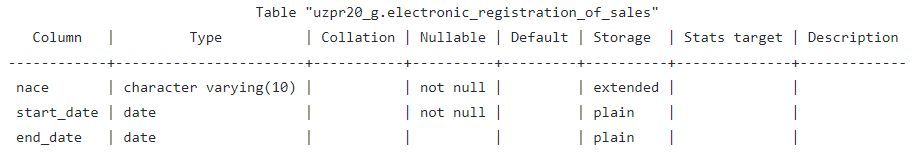
\includegraphics[width=14cm]{eet_tab.jpg}
	\caption{Tabulka electronic registration of sales}
\end{figure}

\subsubsection{Tabulka nace}
\begin{itemize}
\item \textbf{level:} level typu ekonomické činnosti
\item \textbf{code:} kód názvu ekonomické činnosti
\item \textbf{description:} popis ekonomické činnosti
\end{itemize}

\begin{figure}[h!]
	\centering
	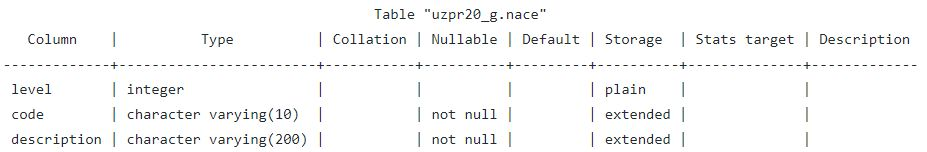
\includegraphics[width=14cm]{nace2_tab.jpg}
	\caption{Tabulka nace}
\end{figure}

\section{Dotazy}
Vytvořené dotazy jsou zaměřené na spuštění evidence elektronických služeb a jejího vlivu ekonomické subjekty. Jsou zde zohledněny 2 vlny spuštění EET (1.12.2016, 3.1.2017) a jejich vliv na ekonomické subjekty s počtem zaměstnanců nižším než 6.

\newpage
\begin{figure}[h!]
	\centering
	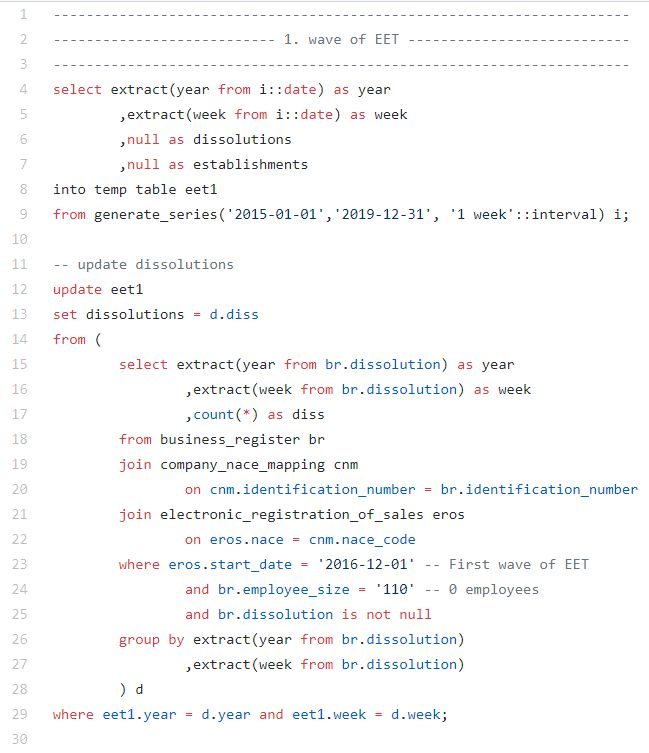
\includegraphics[width=9.6cm]{EET1_A.jpg}

	\centering
	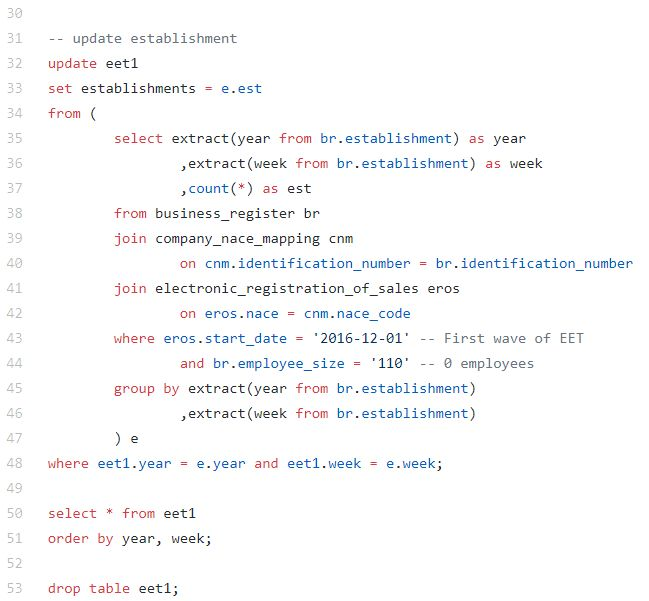
\includegraphics[width=9.5cm]{EET1_A2.jpg}
	\caption{Atributový dotaz vracející počet ekonomických subjektů nově vzniklých a ukončujících svou činnost v intervalu od 1.1.2015 do 31.12.2019 vypisovaný po jednom týdnu. Tyto subjekty podléhají první vlně zavedení EET.}
\end{figure}

\newpage
\begin{figure}[h!]
	\centering
	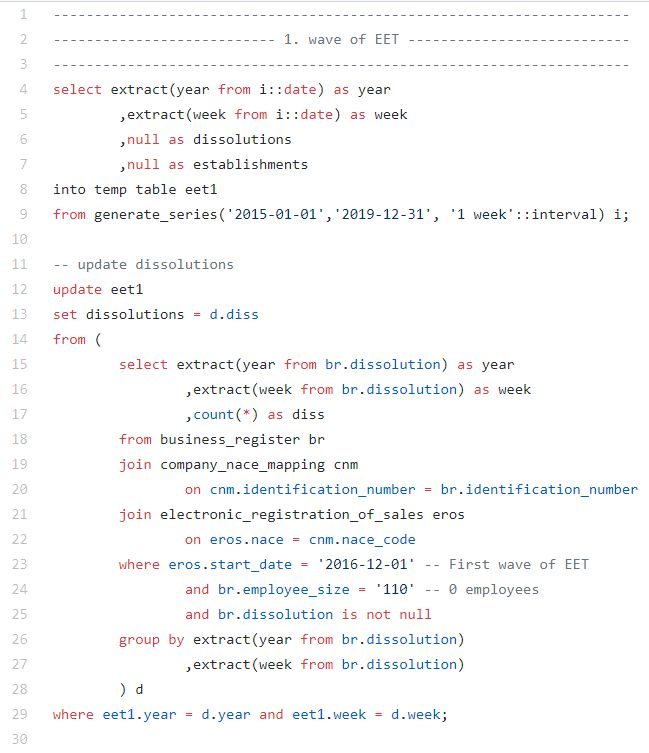
\includegraphics[width=9.6cm]{EET1_A.jpg}
	\caption{Prostorový dotaz vypisující ekonomické subjekty ukončující svoji činnost týden po zavedení první vlny EET.}
\end{figure}

Stejný postup byl použit i pro druhou vlnu EET, kompletní řešení je obsaženo v SQL dávce. 

\newpage
\section{Výstupy projektu}
\begin{figure}[ht]
	\centering
	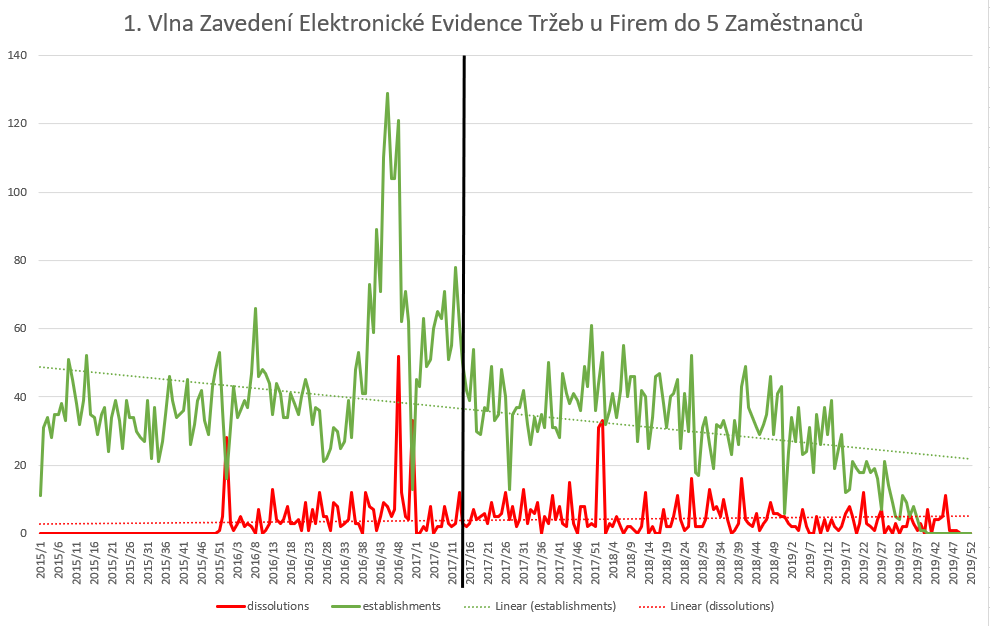
\includegraphics[width=12cm]{1st_do5.png}
	\caption{Graf zobrazující počet vznikajících a zanikajících ekonomických subjektů. Počet zaměstnanců je 5 a méně.}
\end{figure}

\begin{figure}[ht]
	\centering
	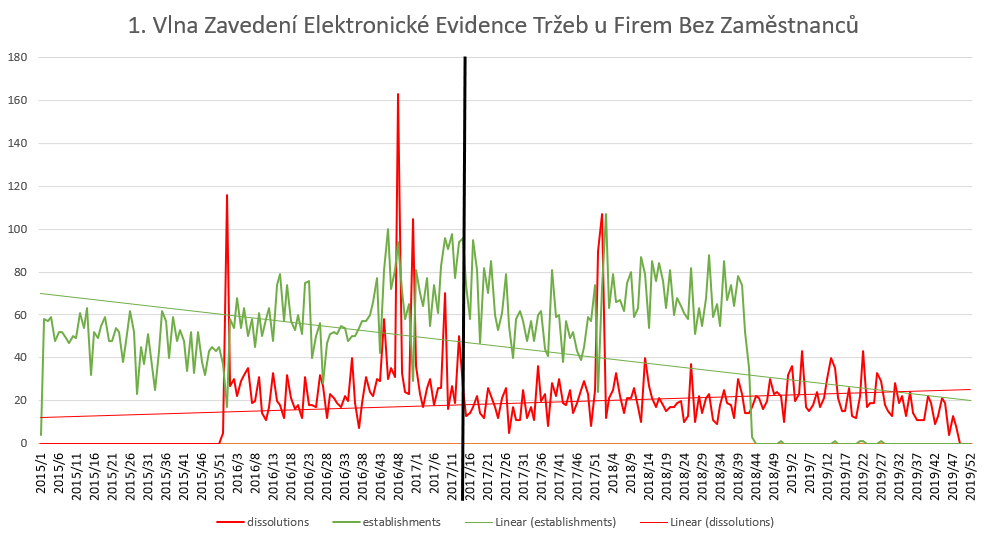
\includegraphics[width=12cm]{1st_bez.png}
	\caption{Graf zobrazující počet vznikajících a zanikajících ekonomických subjektů spadajících do první vlny EET. Počet zaměstnanců je 0.}
\end{figure}

\begin{figure}[ht]
	\centering
	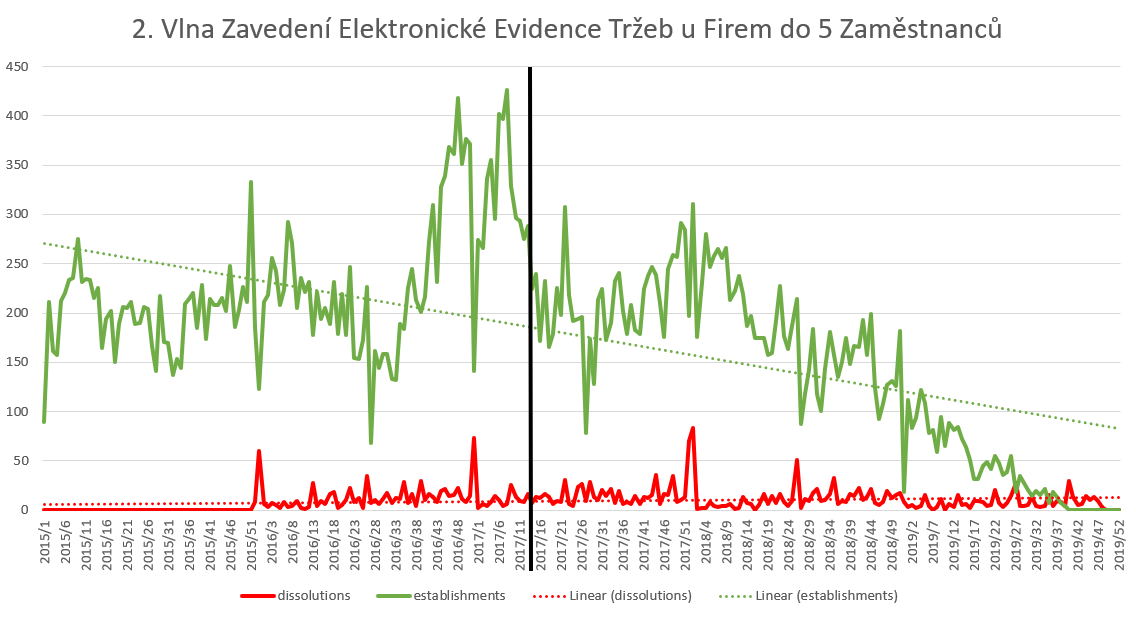
\includegraphics[width=12cm]{2nd_do5.png}
	\caption{Graf zobrazující počet vznikajících a zanikajících ekonomických subjektů spadajících do druhé vlny EET. Počet zaměstnanců je 5 a méně}
\end{figure}

\begin{figure}[ht]
	\centering
	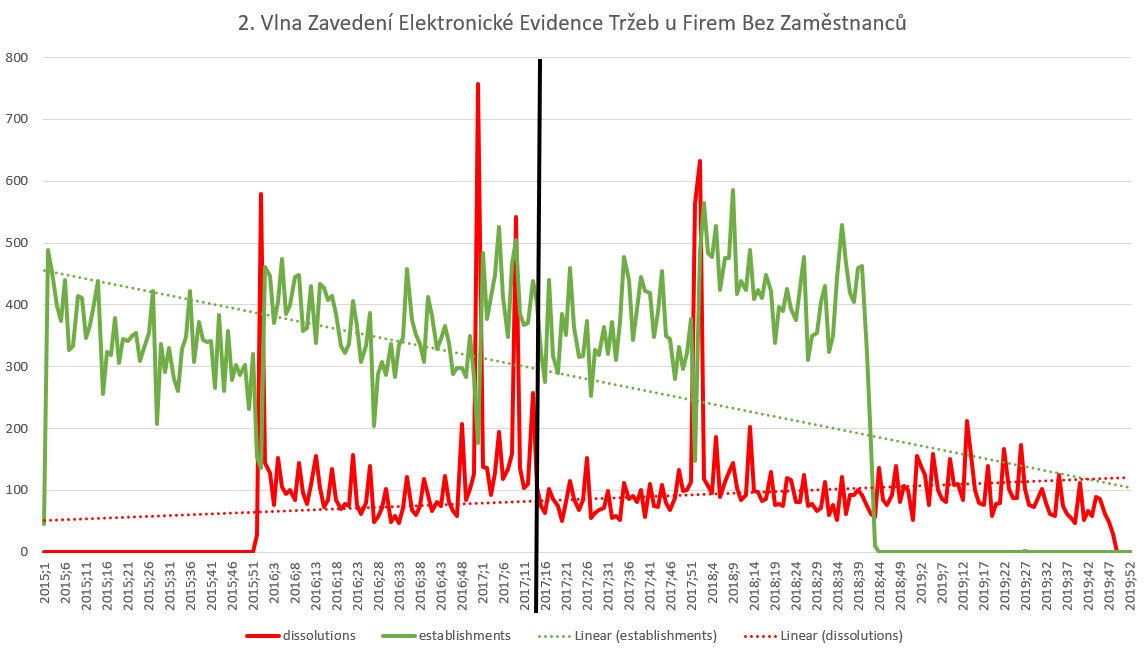
\includegraphics[width=12cm]{2nd_bez.png}
	\caption{Graf zobrazující počet vznikajících a zanikajících ekonomických subjektů spadajících do druhé vlny EET. Počet zaměstnanců je 0.}
\end{figure}

\begin{figure}[ht]
	\centering
	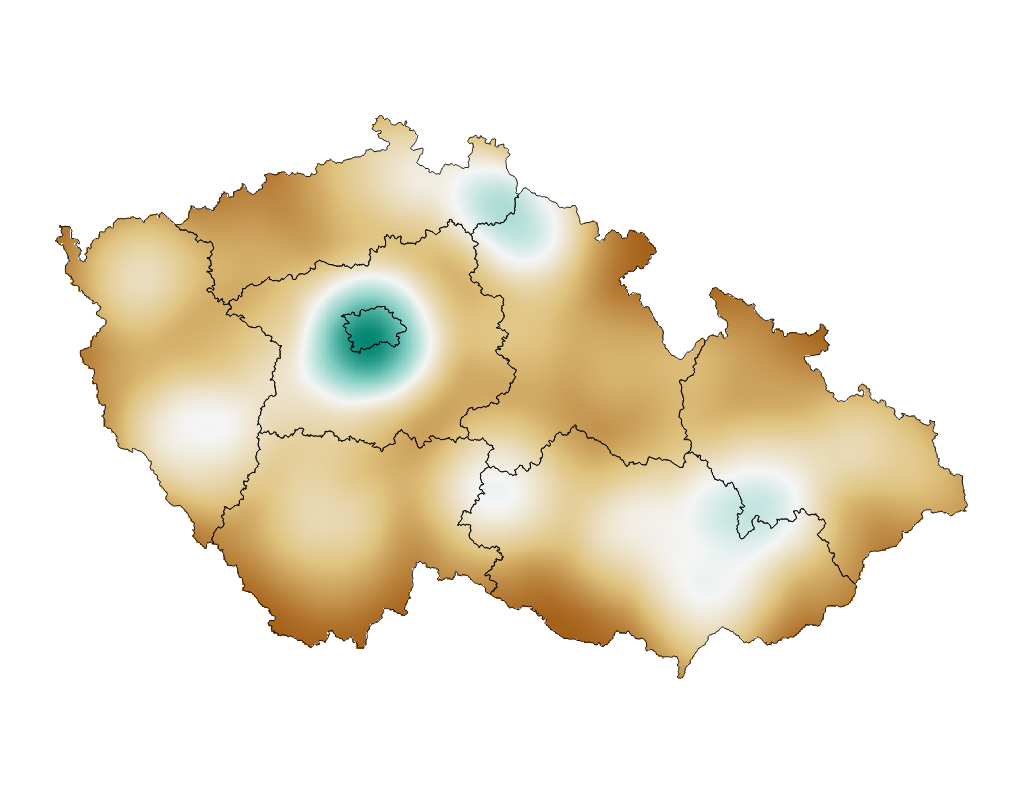
\includegraphics[width=12cm]{1stwave.png}
	\caption{Celoplošná kernel-heat mapa ČR, zobrazující množství ekonomických subjektů ukončující svou činnost v prvním týdnu po zavedení první vlny EET. Počet zaměstnanců je 0.}
\end{figure}

\begin{figure}[ht]
	\centering
	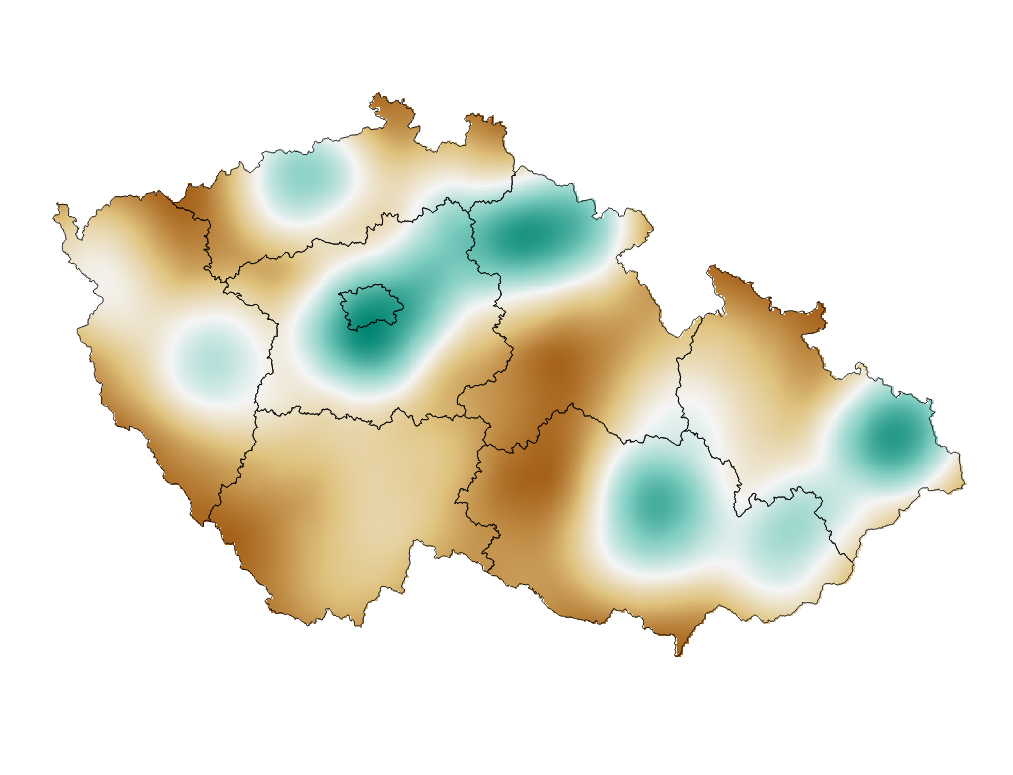
\includegraphics[width=12cm]{2ndwave.png}
	\caption{Celoplošná kernel-heat mapa ČR, zobrazující množství ekonomických subjektů ukončující svou činnost v prvním týdnu po zavedení druhé vlny EET. Počet zaměstnanců je 0.}
\end{figure}

\clearpage
\section{Závěr}
Cílem projektu bylo vytvoření nové databáze pro sledování vnějších a vnitřních vlivů na ekonomické subjekty v celé škále měřítka, od drobných podnikatelů až po korporátní společnosti. Databáze kombinuje atributovou a prostorovou informaci, tudíž nabízí širší perspektivu interpretace dat. Mezi hlavní způsoby využití může být sledování dopadů ve vývoji ekonomiky z hlediska evaluace. Zároveň také může sloužit pro plánování obchodních strategií z hlediska konkurenceschopnosti a pohledávky.\\
\\
Další neméně důležitou částí projektu je způsob jakým byla data získána. Za normálních okolností by data pro tento projekt byla finančně nedostupná. Za pomoci vhodné aplikace byla data získána z veřejných webových aplikací. 

\section{Reference}

\begin{enumerate}

\item \textit{ČESKÝ STATISTICKÝ ÚŘAD} [online], [cit. 2020-2-3]. Dostupné z: \textit{www.czso.cz}

\item \textit{ČÚZK} [online], [cit. 2020-2-3]. Dostupné z: \textit{www.cuzk.cz}

\item \textit{PostgreSQL Tutorial} [online], [cit. 2020-2-3]. Dostupné z: \textit{www.postgresqltutorial.com}

\item \textit{python} [online], [cit. 2020-2-3]. Dostupné z: \textit{www.python.org}

\end{enumerate}
\end{document}



 